\chapter{Einleitung}

\section{Aufgabe/Motivation}

Ziel dieses Versuchs ist die Untersuchung verschiedener Methoden zur Messung von Strom und Spannung in elektrischen Schaltkreisen. Dabei wird insbesondere der Einfluss der verwendeten Messgeräte auf die Messergebnisse betrachtet. Ein Schwerpunkt liegt auf der Analyse der Innenwiderstände sowohl der Spannungsquelle als auch der Messinstrumente, da diese das Messergebnis wesentlich verfälschen können.
Im Rahmen des Versuchs werden zwei Messmethoden miteinander verglichen: die Messung mit einem Drehspulinstrument, das sowohl als Amperemeter als auch als Voltmeter eingesetzt werden kann, sowie die Messung mit einem Kompensator. Zusätzlich wird untersucht, wie sich der Messbereich der Geräte durch den Einsatz zusätzlicher Widerstände erweitern lässt. Ziel ist es, ein Verständnis für die praktische Handhabung von Messgeräten sowie für deren Grenzen und systematische Einflüsse auf die Messergebnisse zu entwickeln.

\section{Physikalische Grundlage}
\cite{skript25}
Grundlage der elektrischen Messungen sind die zusammenhänge zwischen Stromstärke $I$, Spannung $U$ und Widerstand $R$. Diese werden durch das Ohm'sche Gesetz beschrieben:

\begin{equation}
    R = \frac{U}{I}
    \label{eq:ohm}
\end{equation}

Darüber hinaus gelten die Kirchhoff'schen Regeln. Die Knotenregel besagt, dass in einem Knotenpunkt die Summe aller zufließenden und abfließenden Ströme null ist:

\begin{equation}
    \sum_{i} I_i = 0
    \label{eq:knoten}
\end{equation}

Die Maschenregel beschreibt, dass in einer geschlossenen Masche die Summe aller Spannungen null ergibt:

\begin{equation}
    \sum_{i} U_i = 0
    \label{eq:masche}
\end{equation}

Aus diesen Gesetzen lassen sich die Regeln für Reihen- und Paralllelschaltungen von Widerständen ableiten. Für eine Reihenschaltung gilt:

\begin{equation}
    R = \sum_{i} R_i
    \label{eq:reihe}
\end{equation}

Für eine Parallelschaltung folgt:

\begin{equation}
    \frac{1}{R} = \sum_{i} \frac{1}{R_i}
    \label{eq:parallel}
\end{equation}

Reale Spannungsquellen unterscheiden sich von idealen Spannungs Quellen durch das Vorhandensein eines Innenwiderstands $R_i$. Dieser bewirkt, dass die Klemmenspannung $U$ von der entnommenen Stromstärke abhängt:

\begin{equation}
    U = U_q - R_i I
    \label{eq:realquelle}
\end{equation}

mit der Quellenspannung $U_q$. Wird die Spannungsquelle mit einem Lastwiderstand $R_L$ belastet, so ergeben sich für Strom und Spannung:

\begin{equation}
    I = \frac{U_q}{R_i + R_L}
    \label{eq:stromlast}
\end{equation}

\begin{equation}
    U = \frac{U_q R_L}{R_i + R_L}
    \label{eq:spannunglast}
\end{equation}

Damit gilt: Nur wenn $R_i \ll R_L$, entspricht die Klemmenspannung annähernd der Quellenspannung, vgl. \hyperref[eq:realquelle]{Gleichung \ref*{eq:realquelle}}.

\subsection*{Drehspulinstrument}
Zur Strom- und Spannungsmessung wird im Versuch ein Drehspulinstrument verwendet. Dieses besteht aus einer im Feld eines Permanentmagneten drehbar gelagerten Spule, die über eine Rückstellfeder fixiert ist. Fließt Strom durch die Spule, wirkt die Lorentzkraft, sodass ein Drehmoment entsteht. Die Auslenkung ist proportional zur Stromstärke, wodurch die Messung über einen Zeiger sichtbar wird.

Wird das Instrument als Amperemeter genutzt, erfolgt der Anschluss in Reihe. Dabei führt der Innenwiderstand $R_{iA}$ des Instruments zu einer Veringerung der Stromstärke (vgl. \hyperref[eq:stromlast]{Gleichung \ref*{eq:stromlast}}). Um den Messfehler gering zu halten, sollte $R_{iA}$ möglichst klein sein.

\begin{figure}[!ht]
    \centering
    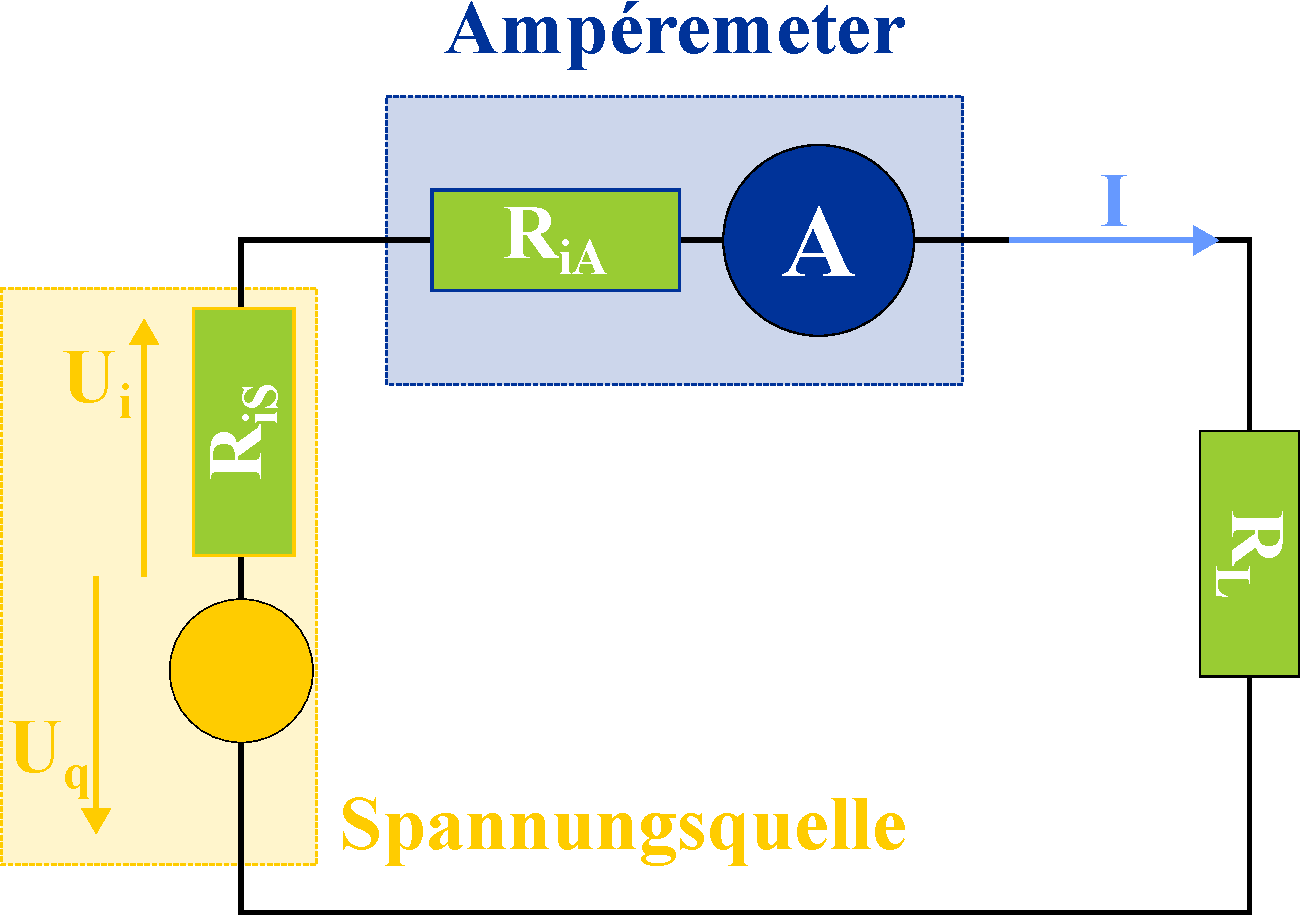
\includegraphics[width=0.45\textwidth]{img/23/AmperemeterSK.pdf}
    \caption{Schaltung des Amperemeters \cite{skript25}}
    \label{fig:amperemeter}
\end{figure}

Wird das Instrument als Voltmeter eingesetzt, erfolgt die Parallelschaltung zum Verbraucher. Hier ist ein hoher Innenwiderstand $R_{iV}$ erwünscht, damit der zusätzliche Stromfluss durch das Messgerät minimal bleibt.

\begin{figure}[!ht]
    \centering
    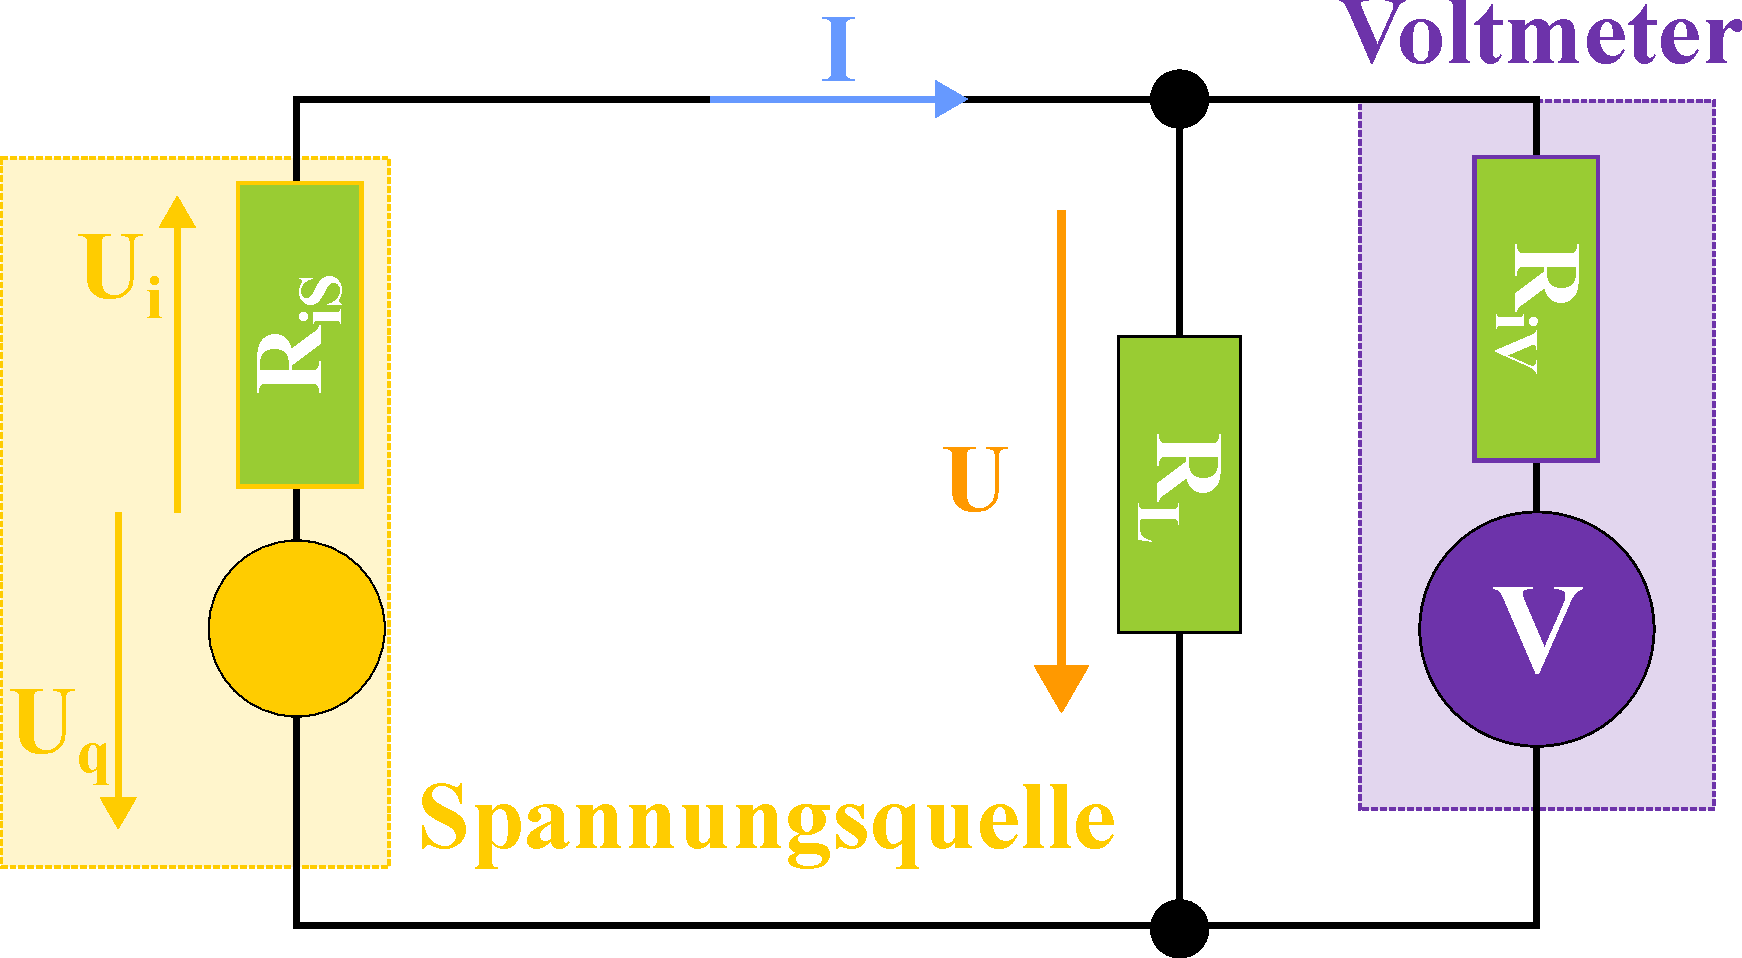
\includegraphics[width=0.45\textwidth]{img/23/VoltmeterSK.pdf}
    \caption{Schaltung des Voltmeters \cite{skript25}}
    \label{fig:voltmeter}
\end{figure}

\subsection*{Kompensator}
Ein alternatives Verfahren stellt die Spannungsmessung mit dem Kompensator dar. Dabei wird der zu messenden Spannung eine bekannte Gegenspannung entgegengesetzt, bis kein Strom mehr fließt. In diesem Fall sind beide Spannungen gleich groß. Aufgrund des hohen Innenwiderstands des Kompensators verursacht dieses Verfahren nur minimale Messfehler und erlaubt eine besonders genaue Spannungsmessung.

Da die Messbereiche von Drehspulinstrumenten begrenzt sind, kann eine Erweiterung durch zusätzliche Widerstände erfolgen. Zur Erweiterung des Strommessbereichs eines Amperemeters wird ein Parallelwiderstand $R_p$ verwendet:

\begin{figure}[!ht]
    \centering
    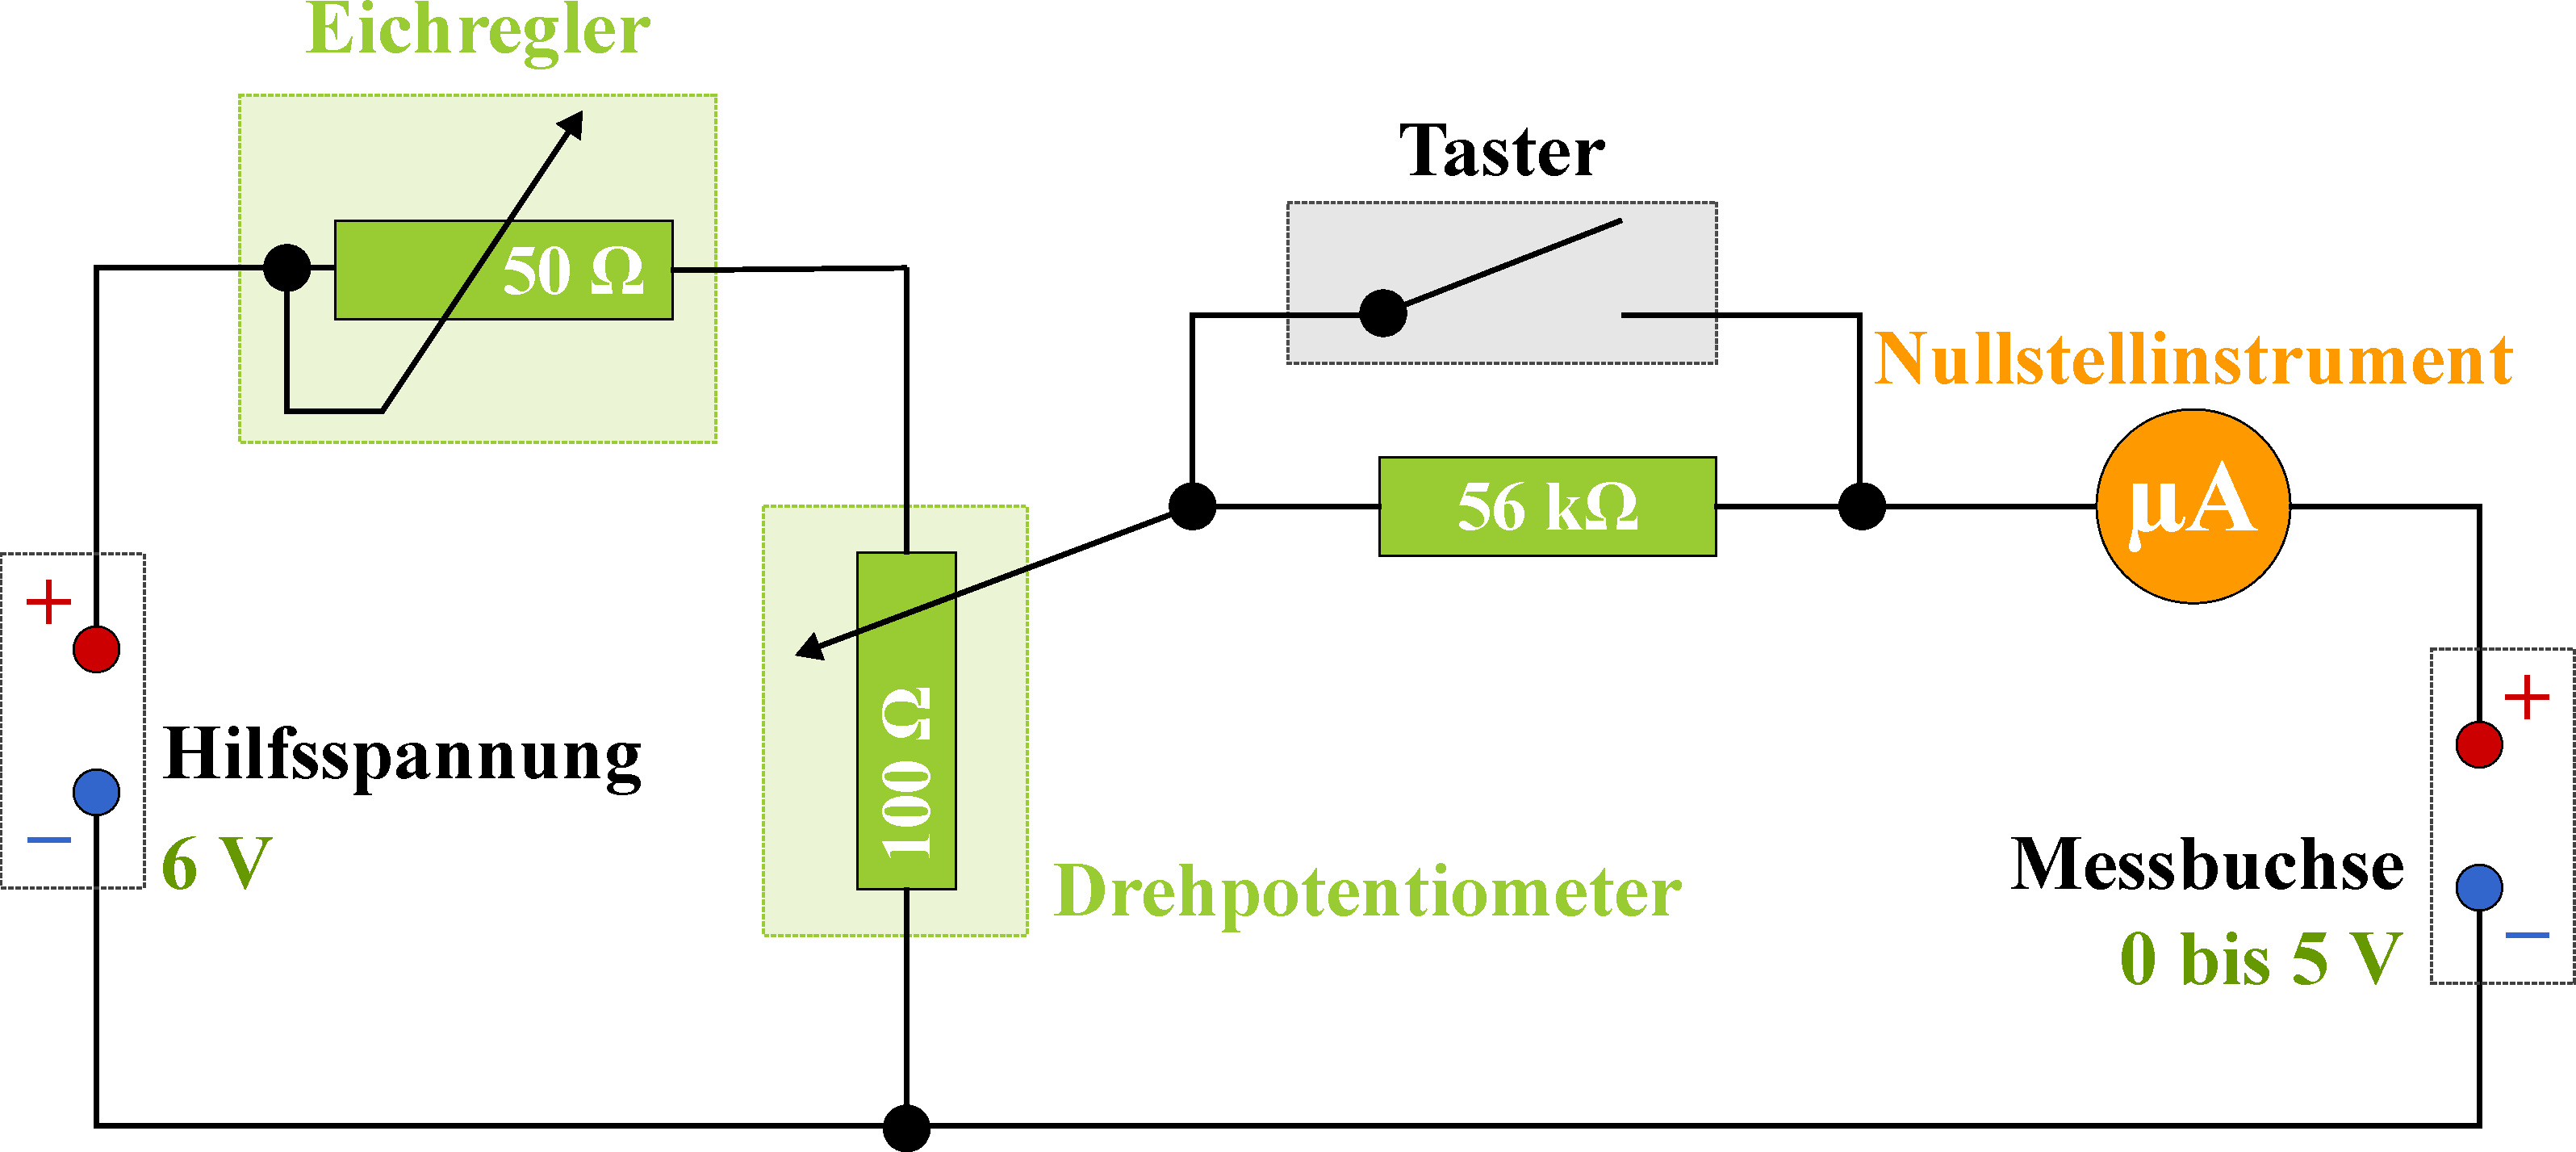
\includegraphics[width=0.5\textwidth]{img/23/kompensaterSK.pdf}
    \caption{Schaltung des Kompensators \cite{skript25}}
    \label{fig:kompensator}
\end{figure}

\begin{equation}
    R_p = \frac{R_i}{f-1}
    \label{eq:stromerw}
\end{equation}

wobei $f$ den Erweiterungsfaktor bezeichnet. Zur Erweiterung des Spannungsmessbereichs eines Voltmeters wird ein Serienwiederstand $R_s$ hinzugefügt:

\begin{equation}
    R_s = R_i (f-1)
    \label{eq:spannungserw}
\end{equation}

Diese Schaltungen erlauben es, auch Ströme und Spannungen zu messen, die den ursprünglichen Messbereich des Geräts überschreiten.